Intuitivamente, podemos pensar en un \textit{grafo simple} como una colección de círculos o puntos llamados \textit{vértices}, conectados con segmentos que llamamos \textit{aristas}.
\begin{figure}[H]
\centering
\resizebox{0.3\textwidth}{!}{
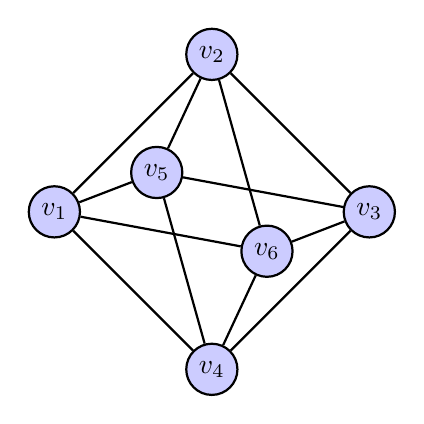
\begin{tikzpicture}[
  scale=1.0,
  vnode/.style={circle, draw=black, fill=blue!20, thick, inner sep=0pt, minimum size=6.5mm},
  edge/.style={thick, draw=black}
]
  % Vértices exteriores (cuadrado C4)
  \node[vnode] (v1) at (-2, 0) {$v_1$};
  \node[vnode] (v2) at (0, 2) {$v_2$};
  \node[vnode] (v3) at (2, 0) {$v_3$};
  \node[vnode] (v4) at (0, -2) {$v_4$};

  % Vértices polo interior/exterior (conectados a todo el C4)
  \node[vnode] (v5) at (-0.7, 0.5) {$v_5$};
  \node[vnode] (v6) at (0.7, -0.5) {$v_6$};

  % Aristas del cuadrado exterior
  \draw[edge] (v1) -- (v2) -- (v3) -- (v4) -- (v1);

  % Conexiones del vértice v5 (polo superior/interior)
  \draw[edge] (v5) -- (v1);
  \draw[edge] (v5) -- (v2);
  \draw[edge] (v5) -- (v3);
  \draw[edge] (v5) -- (v4);

  % Conexiones del vértice v6 (polo inferior/interior)
  \draw[edge] (v6) -- (v1);
  \draw[edge] (v6) -- (v2);
  \draw[edge] (v6) -- (v3);
  \draw[edge] (v6) -- (v4);

\end{tikzpicture}}%
\caption{Un grafo simple}
\end{figure}

En los grafos simples cada arista conecta exactamente dos vértices, de modo que no puede haber aristas que conecten un vértice consigo mismo, ni puede haber más de una arista entre dos vértices. Siguiendo a \cite{Foulds1991}, \cite{Gross2006} y \cite{Pirzada2007}, vemos que, a nivel práctico, los grafos simples son la herramienta estándar para modelar ciertas redes de contactos o relaciones sociales entre personas, organizar la asignación óptima de personal a diferentes tareas y planificar la infraestructura de redes físicas de computadores o servidores. También se utilizan para resolver problemas de asignación de frecuencias en antenas de telefonía móvil evitando interferencias electrónicas, e incluso en biología computacional y ciberseguridad para detectar conflictos genéticos o aislar virus informáticos en servidores clave mediante el análisis de coberturas mínimas. Según las fuentes, la gran ventaja de los grafos simples radica en la limpieza y eficiencia de su estructura. Al no admitir conexiones repetidas ni bucles sobre un mismo punto, pueden almacenarse en computadoras mediante matrices o listas de conexiones muy compactas, lo que mejora significativamente el uso de memoria y a su vez facilita el diseño de algoritmos de búsqueda y optimización extremadamente rápidos.\\\\
Una ligera variante en la noción de grafo simple la presentan los llamados \textit{grafos orientados}. Podemos pensar en un grafo orientado como en un grafo simple en el cual a cada arista se le asigna una ``dirección'', de modo que ahora tenemos registro del vértice del cual ``sale'' una arista y al cual ``llega''. Las aristas son ahora representadas por flechas apuntando desde el vértice de salida al vértice de llegada. Si el grafo orientado $D$ resulta de asignar dirección a las aristas del grafo simple $G$, decimos que $D$ es una \textit{orientación} de G.
\begin{figure}[H]
   \centering
   \resizebox{0.4\textwidth}{!}{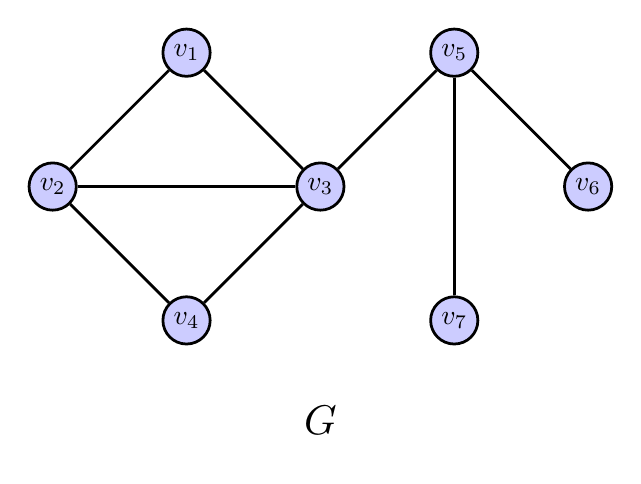
\begin{tikzpicture}[
  scale=0.85, 
  auto=left,
  every node/.style={circle, fill=blue!20, draw=black, line width=1pt, inner sep=2pt, minimum size=6mm}
]

  % Vértices según la disposición del dibujo
  \node (v1) at (2,4) {$v_1$};
  \node (v2) at (0,2) {$v_2$};
  \node (v3) at (4,2) {$v_3$};
  \node (v4) at (2,0) {$v_4$};
  \node (v5) at (6,4) {$v_5$};
  \node (v6) at (8,2) {$v_6$};
  \node (v7) at (6,0) {$v_7$};

  % Aristas de la sección izquierda (entre v1, v2, v3, v4)
  \draw[line width=1pt] (v1) -- (v2);
  \draw[line width=1pt] (v1) -- (v3);
  \draw[line width=1pt] (v2) -- (v3);
  \draw[line width=1pt] (v2) -- (v4);
  \draw[line width=1pt] (v4) -- (v3);

  % Conexión puente (v3 -- v5)
  \draw[line width=1pt] (v3) -- (v5);

  % Aristas de la estrella en v5 (v5 -- v6, v5 -- v7)
  \draw[line width=1pt] (v5) -- (v6);
  \draw[line width=1pt] (v5) -- (v7);

   
  \node[draw=none, fill=none, scale=1.5] at (4,-1.5) {$G$};
\end{tikzpicture}
} \hspace{2em}
   \resizebox{0.4\textwidth}{!}{% Recuerda incluir en el preámbulo:
% \usetikzlibrary{arrows.meta, babel}

\begin{tikzpicture}[
  scale=0.85, 
  auto=left,
  >={Stealth[length=2.5mm]},
  every node/.style={circle, fill=blue!20, draw=black, line width=1pt, inner sep=2pt, minimum size=6mm},
  flecha/.style={->, line width=1pt}
]

  % Vértices según la disposición del dibujo
  \node (v1) at (2,4) {$v_1$};
  \node (v2) at (0,2) {$v_2$};
  \node (v3) at (4,2) {$v_3$};
  \node (v4) at (2,0) {$v_4$};
  \node (v5) at (6,4) {$v_5$};
  \node (v6) at (8,2) {$v_6$};
  \node (v7) at (6,0) {$v_7$};

  % Aristas orientadas del bloque izquierdo
  \draw[flecha] (v2) -- (v1);
  \draw[flecha] (v1) -- (v3);
  \draw[flecha] (v2) -- (v3);
  \draw[flecha] (v2) -- (v4);
  \draw[flecha] (v4) -- (v3);

  % Conexión puente orientada
  \draw[flecha] (v3) -- (v5);

  % Aristas orientadas (v6 -> v5 invertida)
  \draw[flecha] (v6) -- (v5);
  \draw[flecha] (v5) -- (v7);

  \node[draw=none, fill=none, scale=1.5] at (4,-1.5) {$D$};
\end{tikzpicture}
} 
   \caption{$D$ es una orientación de $G$}
\end{figure}
\clearpage
En \cite{Foulds1991} y \cite{Roberts1978} se nos muestra que esta noción de dirección única permite organizar de forma eficiente el flujo vehicular en ciudades mediante calles de un solo sentido sin generar zonas atrapadas o inaccesibles, o representar las jerarquías de victoria y derrota en competencias de tipo ``todos contra todos''. También se nos afirma que el beneficio de un grafo dirigido frente al grafo simple es que añade una jerarquía a las conexiones; sin embargo, al prohibir arcos de ida y vuelta simultáneos entre los mismos dos puntos, conserva una estructura ligera que aún simplifica los cálculos.\\\\
Permitiendo más de una arista entre dos vértices en un grafo orientado, así como aristas de un vértice en sí mismo, obtenemos la noción de \textit{grafo dirigido} o \textit{digrafo}. Las aristas que conectan un mismo par de vértices (sin importar en qué dirección lo hagan) son llamadas \textit{aristas múltiples}. Si un conjunto de aristas múltiples tiene la misma dirección, estas son llamadas \textit{aristas paralelas}. Las aristas que unen un vétice consigo mismo son llamados \textit{bucles}. En la representación de un grafo dirigido solemos curvar ligeramente las aristas múltiples para evitar que estas se superpongan. Ahora, también etiquetamos las aristas del grafo dirigido para poder hacer distinción entre aristas paralelas.
\begin{figure}[H]
  \centering
    \resizebox{0.5\textwidth}{!}{% Recuerda incluir en el preámbulo:
% \usetikzlibrary{arrows.meta, babel}

\begin{tikzpicture}[
  scale=0.85, 
  auto=left,
  >={Stealth[length=2.5mm]},
  every node/.style={circle, fill=blue!20, draw=black, line width=1pt, inner sep=2pt, minimum size=6mm}
]

  % Posicionamiento de vértices
  \node (v1) at (3,6) {$v_1$};
  \node (v2) at (0,4) {$v_2$};
  \node (v3) at (6,4) {$v_3$};
  \node (v4) at (3,3) {$v_4$};
  \node (v5) at (0,1) {$v_5$};
  \node (v6) at (6,1) {$v_6$};
  \node (v7) at (9,1.5) {$v_7$};

  % Bucles en v1 (e1 y e2)
  % e1 bajado un poco más (yshift=-5pt)
  \path[->, line width=1pt] (v1) edge[loop above, out=120, in=60, looseness=8] node[draw=none, fill=none, above] {$e_1$} (v1);
  \path[->, line width=1pt] (v1) edge[loop above, out=150, in=30, looseness=18] node[draw=none, fill=none, above] {$e_2$} (v1);

  % Conexiones v1 <-> v2
  \draw[->, line width=1pt] (v2) to[bend left=15] node[draw=none, fill=none, above] {$e_3$} (v1);
  \draw[->, line width=1pt] (v1) to[bend left=15] node[draw=none, fill=none, below] {$e_4$} (v2);

  % Arista v1 -> v4
  \draw[->, line width=1pt] (v1) -- node[draw=none, fill=none, right] {$e_5$} (v4);

  % Arista v4 -> v5
  \draw[->, line width=1pt] (v4) -- node[draw=none, fill=none, above] {$e_6$} (v5);

  % Bucle en v5 (e7) - Ajustado para alejarlo menos (yshift/xshift reducido a -2pt)
  \path[->, line width=1pt] (v5) edge[loop left, out=210, in=150, looseness=8] node[draw=none, fill=none, xshift=-1pt, yshift=-1pt] {$e_7$} (v5);

  % Múltiples aristas v4 -> v6 (e8, e9, e10)
  \draw[->, line width=1pt] (v4) to[bend left=10] node[draw=none, fill=none, above] {$e_8$} (v6);
  \draw[->, line width=1pt] (v4) to[bend right=25] node[draw=none, fill=none, below] {$e_9$} (v6);
  \draw[->, line width=1pt] (v4) to[bend right=60] node[draw=none, fill=none, below] {$e_{10}$} (v6);

  % Arista v6 -> v4 (e11)
  \draw[->, line width=1pt] (v6) to[bend right=45] node[draw=none, fill=none, above] {$e_{11}$} (v4);

  % Arista v7 -> v3 (e12) - Mantiene orientación horizontal/vertical (sin sloped) y centrada con pos=0.5
  \draw[->, line width=1pt] (v7) -- node[draw=none, fill=none, pos=0.35, above] {$e_{12}$} (v3);

\end{tikzpicture}
} 
  \caption{Un grafo dirigido}
  \label{fig:digrafo}
\end{figure}
En el grafo dirigido de la \Cref{fig:digrafo} podemos señalar, por ejemplo, que $e_1, e_2$ y $e_7$ son bucles, $e_3$ y $e_4$ son aristas múltiples entre $v_1$ y $v_2$, y $e_8,e_9$ y $e_{10}$ son aristas paralelas. Tal como se señala en \cite{Foulds1991}, \cite{Gross2006} y \cite{Roberts1978}, esta flexibilidad hace que los digrafos sean indispensables para coordinar las etapas de proyectos complejos, determinando qué actividades deben terminarse antes de iniciar otras, como reconstruir la secuencia original de fragmentos de ADN o ARN en biología y modelar sistemas con probabilidades de transición entre estados en economía y sociología, por ejemplo. Las fuentes nos muestran que la ventaja de los grafos dirigidos sobre los grafos orientados es que permiten flujos bidireccionales y recorridos que vuelven al mismo punto, algo esencial para representar procesos dinámicos con retroalimentación o ciclos de repetición.\\\\
Si en un grafo dirigido ignoramos la dirección de sus aristas, obtenemos un \textit{multigrafo}.
\begin{figure}[H]
  \centering
  \resizebox{0.45\textwidth}{!}{% Recuerda incluir en el preámbulo:
% \usetikzlibrary{arrows.meta, babel}

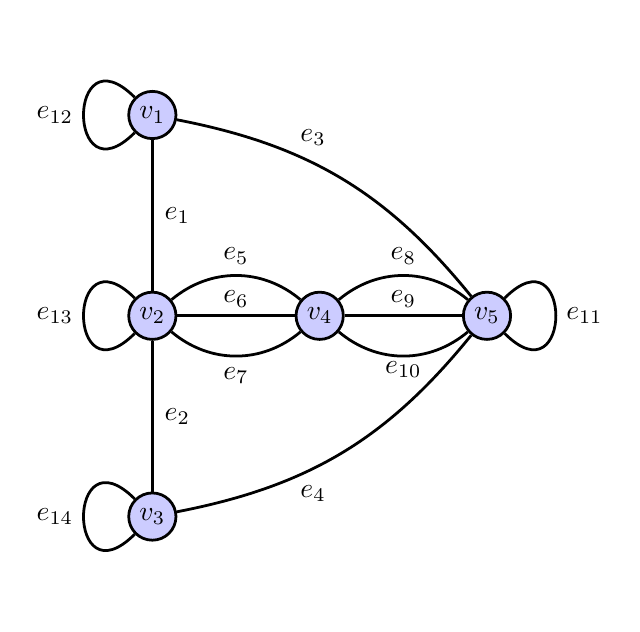
\begin{tikzpicture}[
  scale=0.85, 
  auto=left,
  every node/.style={circle, fill=blue!20, draw=black, line width=1pt, inner sep=2pt, minimum size=6mm}
]

  % Posicionamiento horizontal de vértices
  \node (v1) at (0,3) {$v_1$};
  \node (v3) at (0,-3) {$v_3$};
  \node (v2) at (0,0) {$v_2$};
  \node (v4) at (2.5,0) {$v_4$};
  \node (v5) at (5,0) {$v_5$};

  % Bucles en v1, v2 y v3
  \path[line width=1pt] (v1) edge[loop left, out=135, in=225, looseness=7] node[draw=none, fill=none, left, inner sep=2pt] {$e_{12}$} (v1);
  \path[line width=1pt] (v2) edge[loop left, out=135, in=225, looseness=7] node[draw=none, fill=none, left, inner sep=2pt] {$e_{13}$} (v2);
  \path[line width=1pt] (v3) edge[loop left, out=135, in=225, looseness=7] node[draw=none, fill=none, left, inner sep=2pt] {$e_{14}$} (v3);

  % Aristas verticales iniciales
  \draw[line width=1pt] (v1) -- node[draw=none, fill=none, right, inner sep=1pt] {$e_1$} (v2);
  \draw[line width=1pt] (v2) -- node[draw=none, fill=none, right, inner sep=1pt] {$e_2$} (v3);

  % Conexiones curvas v1 -> v5 y v3 -> v5
  \draw[line width=1pt] (v1) to[bend left=20] node[draw=none, fill=none, above, inner sep=1pt, pos=0.4] {$e_3$} (v5);
  \draw[line width=1pt] (v3) to[bend right=20] node[draw=none, fill=none, below, inner sep=1pt, pos=0.4] {$e_4$} (v5);

  % Múltiples aristas entre v2 y v4
  \draw[line width=1pt] (v2) to[bend left=40] node[draw=none, fill=none, above, yshift=-2pt] {$e_5$} (v4);
  \draw[line width=1pt] (v2) -- node[draw=none, fill=none, above, yshift=-3pt] {$e_6$} (v4);
  \draw[line width=1pt] (v2) to[bend right=40] node[draw=none, fill=none, below, yshift=2pt] {$e_7$} (v4);

  % Múltiples aristas entre v4 y v5
  \draw[line width=1pt] (v4) to[bend left=40] node[draw=none, fill=none, above, yshift=-2pt] {$e_8$} (v5);
  \draw[line width=1pt] (v4) -- node[draw=none, fill=none, above, yshift=-3pt] {$e_9$} (v5);
  \draw[line width=1pt] (v4) to[bend right=40] node[draw=none, fill=none, below, yshift=5.5pt] {$e_{10}$} (v5);

  % Bucle en v5
  \path[line width=1pt] (v5) edge[loop right, out=45, in=-45, looseness=7] node[draw=none, fill=none, right, pos=0.5, inner sep=2pt] {$e_{11}$} (v5);

\end{tikzpicture}
} 
  \caption{Un multigrafo}
  \label{fig:multigrafo}
\end{figure}
En un multigrafo aún se permiten aristas múltiples entre vértices, así como bucles. En el multigrafo de la \Cref{fig:multigrafo} podemos ver, por ejemplo, que $e_8,e_9$ y $e_{10}$ son aristas múltiples entre $v_4$ y $v_5$, que $e_{12}$ es un bucle sobre $v_1$ y que $e_{14}$ es un bucle sobre $v_3$. De acuerdo con \cite{Andrei2008}, \cite{Butler2023}, \cite{Gross2006} y \cite{Shafie2012}, los multigrafos se aplican con éxito en el análisis de redes sociales para estudiar simultáneamente distintos tipos de lazos entre las mismas personas (como amistad, trabajo o préstamos de dinero), en la representación de redes de transporte con varias alternativas paralelas (como tren y autobús entre dos estaciones) y en química, para describir enlaces moleculares múltiples, entre otros. Se menciona que la principal ventaja de los multigrafos reside en que pueden registrar varios canales de interacción al mismo tiempo, sin necesidad de simplificarlos o fusionarlos en un solo enlace, preservando la riqueza del fenómeno real.\clearpage
Si ahora permitimos que las aristas sean subconjuntos de vértices no vacíos, y de cualquier cardinalidad, obtenemos la noción de \textit{hipergrafo}. Las aristas de un hipergrafo se representan como diagramas de Venn, encerrando únicamente los vértices que contiene.
\begin{figure}[H]
  \centering
    \resizebox{0.6\textwidth}{!}{% Recuerda incluir en el preámbulo:
% \usetikzlibrary{babel}

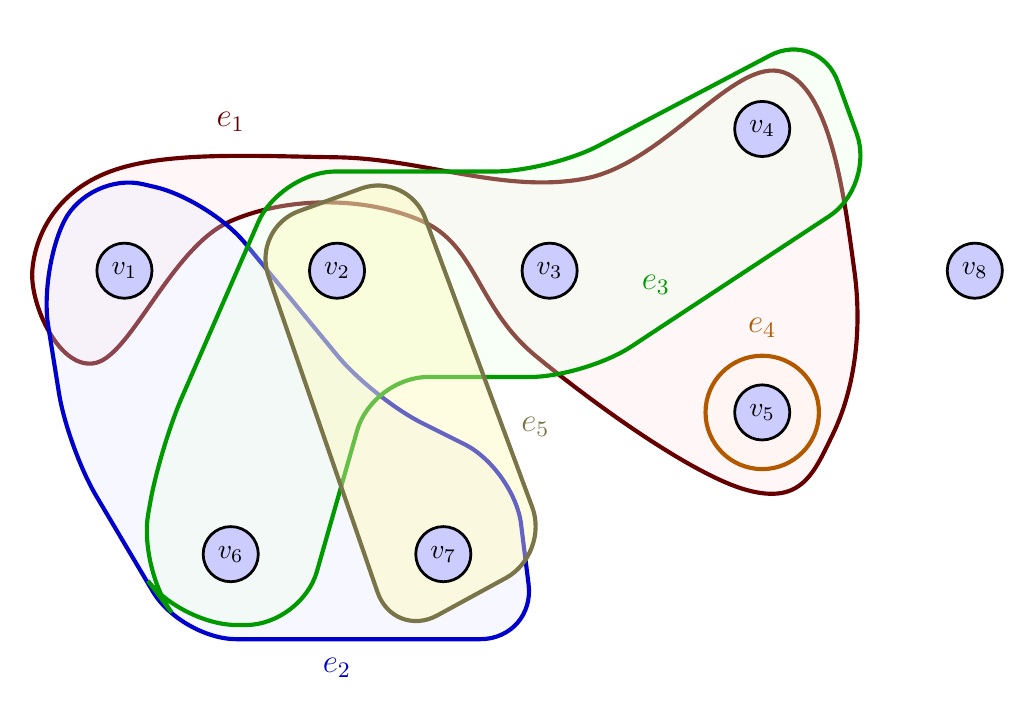
\begin{tikzpicture}[
  scale=0.9,
  every node/.style={circle, fill=blue!20, draw=black, line width=1pt, inner sep=2pt, minimum size=7mm}
]

  % ==========================================
  % 1. HIPERARISTAS (dibujadas al fondo)
  % ==========================================
  
  % e1 = {v1, v3, v4, v5} (Rojo oscuro - trazado orgánico y suave)
  \draw[red!40!black, line width=1.5pt, fill=red!10, fill opacity=0.3]
    plot [smooth cycle, tension=0.65] coordinates {
      (-1.3, 3.0)
      (-0.2, 4.4)
      (3.0, 4.6)
      (6.5, 4.3)
      (9.3, 5.8)
      (10.3, 3.0)
      (10.0, 0.7)
      (8.8, -0.1)
      (5.8, 1.8)
      (4.2, 3.7)
      (1.5, 3.7)
      (-0.4, 1.7)
    };
  \node[draw=none, fill=none, red!40!black, font=\large] at (1.5, 5.1) {$e_1$};

  % e2 = {v1, v6, v7} (Azul)
  \draw[blue!80!black, line width=1.5pt, fill=blue!10, fill opacity=0.3, rounded corners=20pt]
    (-1.2, 3) -- (-0.5, 4.4) -- (1.2, 4) -- (3.5, 1.2) -- (5.5, 0.2) -- 
    (5.8, -2.2) -- (0.8, -2.2) -- (-0.8, 0.5) -- cycle;
  \node[draw=none, fill=none, blue!80!black, font=\large] at (3, -2.6) {$e_2$};

  % e3 = {v2, v3, v4, v6} (Verde)
  \draw[green!60!black, line width=1.5pt, fill=green!10, fill opacity=0.3, rounded corners=20pt]
    (0.2, -1.2) -- (0.5, 0.5) -- (2.2, 4.4) -- (6, 4.4) -- (9.8, 6.4) -- 
    (10.6, 4.2) -- (6.5, 1.5) -- (3.5, 1.5) -- (2.5, -2) -- (0.8, -2) -- cycle;
  \node[draw=none, fill=none, green!60!black, font=\large] at (7.5, 2.8) {$e_3$};

  % e5 = {v2, v7} (Amarillo oscuro/Dorado)
  \draw[yellow!40!black, line width=1.5pt, fill=yellow!30, fill opacity=0.4, rounded corners=18pt]
    (1.8, 3.6) -- (4, 4.4) -- (6, -1) -- (3.8, -2.2) -- cycle;
  \node[draw=none, fill=none, yellow!40!black, font=\large] at (5.8, 0.8) {$e_5$};

  % e4 = {v5} (Naranja)
  \draw[orange!70!black, line width=1.5pt, fill=orange!10, fill opacity=0.3]
    (9,1) circle (8mm);
  \node[draw=none, fill=none, orange!70!black, font=\large] at (9, 2.2) {$e_4$};


  % ==========================================
  % 2. VÉRTICES (dibujados sobre las áreas)
  % ==========================================
  \node (v1) at (0,3) {$v_1$};
  \node (v2) at (3,3) {$v_2$};
  \node (v3) at (6,3) {$v_3$};
  \node (v4) at (9,5) {$v_4$};
  \node (v5) at (9,1) {$v_5$};
  \node (v6) at (1.5,-1) {$v_6$};
  \node (v7) at (4.5,-1) {$v_7$};
  \node (v8) at (12,3) {$v_8$};

\end{tikzpicture}
} 
  \caption{Un hipergrafo}
\end{figure}
Según lo señalado en \cite{Bretto2013} y \cite{Molnar2014}, los hipergrafos son muy útiles en informática para diseñar y organizar grandes bases de datos relacionales, coordinar horarios concurrentes sin solapamientos y analizar colaboraciones de grupo en redes de personas (como comités o artículos científicos escritos por múltiples autores). Nos muestran que el máximo beneficio de este tipo de grafos radica en romper la barrera del enlace por parejas, agrupando a un número arbitrario de participantes en una misma relación e independizando al modelo de simplificaciones bidireccionales o binarias artificiales.
